\section{系统问题总结}
\subsection{关于系统软关机复位问题}
Q:系统软关机使用内置触摸和普通IO关机,开机时\emphasizebox{reset}位置有什么不同?
\begin{itemize}
    \item 普通IO关机,P11系统会掉电,指剩下P33维持电压,开机\emphasizebox{reset}是从\emphasizebox{maskrom}的\emphasizebox{startup}开始;
    \item 使用内置触摸关机,P11系统维持电源工作,这是关机之后还会大几\emphasizebox{uA}的原因,开机\emphasizebox{reset}也是从\emphasizebox{maskrom}的\emphasizebox{Startup}开始;
\end{itemize}

\subsection{关于使用内置触摸开机ROM中IO状态恢复出错问题}
Q:当使用内置触摸开机时,发现\emphasizebox{PC3 IO}变为输出低状态,关机之前在mask\_IO中已经把IO状态设置为高阻?
\begin{itemize}
    \item 当使用\emphasizebox{LPCTMU}关机时,会使用\emphasizebox{PLCNT}模块,配置了\emphasizebox{P3\_PCNT\_SET0}和\emphasizebox{P3\_PCNT\_SET1}两个寄存器,\emphasizebox{PC3 IO}状态正好配置了3,导致在mask恢复IO时设置为输出0状态;
    \item 解决办法:在\emphasizebox{soft\_off\_enter}和\emphasizebox{soft\_off\_exit}时加入\emphasizebox{save}和\emphasizebox{recover}流程即可。
\end{itemize}

\subsection{br28 ass ASS\_CLK\_CON bit7写完和读出来不一样问题(bit5)}
问题:在写ASS\_CLK\_CON的bit7置1时,写完读出来是0x40,再写bit7置0时,读出来时0x20;

解释:由于bit5没有用到,cpu读会移位,在软件层面第一次写bit7置1时,cpu行为:
\begin{myccode}[caption={bit7置1 cpu行为}]
    {
        int bak = 0;
        bak = ASS_CLK_CON;
        bak |= BIT(7);
        ASS_CLK_CON = bak;
    }
\end{myccode}
由于bit5没用到,在cpu读时,bit6变bit5,bit7变bit6,因此写完bit7之后,读出来是0b0100,0000 = 0x40,再把bit7写0时,cpu行为:
\begin{myccode}[caption={bit7置0 cpu行为}]
    {
        int bak = 0;
        bak = ASS_CLK_CON;  //此时bak = 0b0100,0000
        bak &= ~BIT(7);     //此时bak = 0b0100,0000
        ASS_CLK_CON = bak;  //写bit7为0无效;
    }
\end{myccode}
下次再写bit7,将会读回来是0b1100, 0000 = 0xC0,导致出错,硬件Bug;

\subsection{br34 RVDD电压要大于等于DVDD问题}
如果RVDD < DVDD时,有的板子会出现程序跑到某个ram地址出现非对齐访问异常问题。
\begin{figure}[H]
\centering
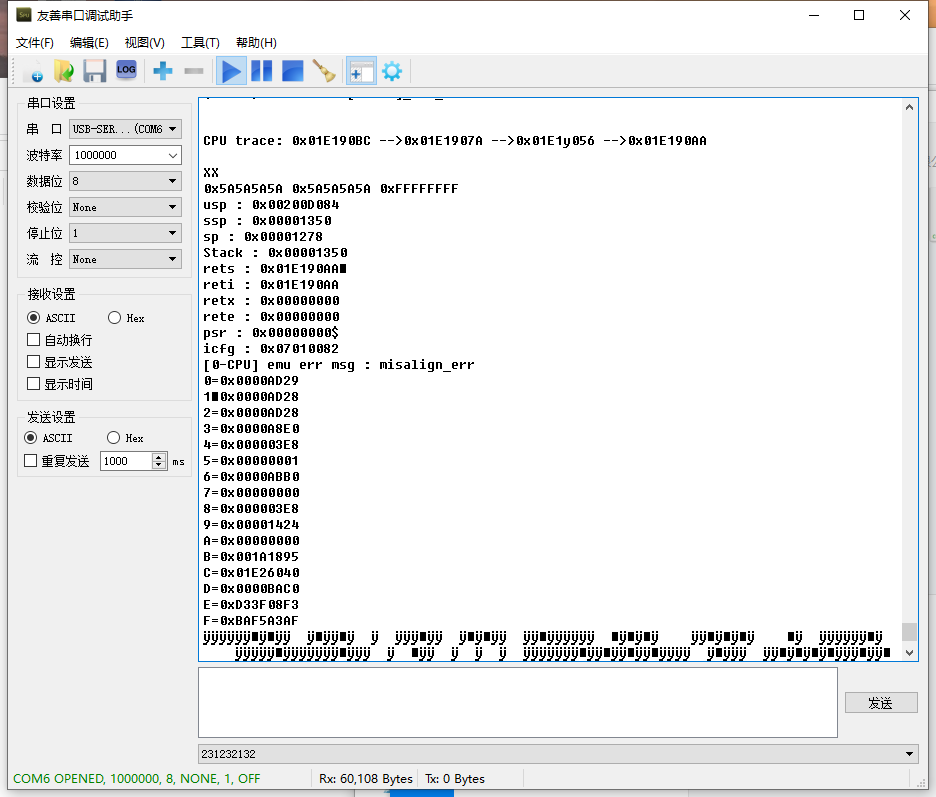
\includegraphics[height=8cm]{rvdd_question.png}
\caption{异常打印}
\label{fig:rvdd_exeception}
\end{figure}
注意:RVDD >= DVDD。


\subsection{有符号数十六进制转十进制计算方法}
计算机内存数值存储方式
1)原码:一个数的原码(原始的二进制码)有如下特点:
\begin{itemize}
\item 最高位做为符号位,0表示正,1表示负
\item 其它数值部分就是数值本身绝对值的二进制数
\item 负数的原码是在其绝对值的基础上,最高位变为1
\item 原码表示法简单易懂,与带符号数本身转换方便,只要符号还原即可,但当两个正数相减或不同符号数相加时,必须比较两个数哪个绝对值大,才能决定谁减谁,才能确定结果是正还是负,所以原码不便于加减运算
\end{itemize}

2)反码
\begin{itemize}
\item 对于正数,反码与原码相同
\item 对于负数,符号位不变,其它部分取反(1变0,0变1)
\item 反码运算也不方便,通常用来作为求补码的中间过渡
\end{itemize}

3)补码
\begin{itemize}
\item 对于正数,原码、反码、补码相同
\item 对于负数,其补码为它的反码加1
\item 补码符号位不动,其它位求反,最后整个数加1,得到原码
\item 在计算机系统中,数值一律用补码来存储
\end{itemize}

4)计算机系统中,数值一律用补码来存储,主要原因是:
\begin{itemize}
\item 统一了零的编码,0在计算机中存储的方式:
\begin{myccode}[caption=zero 编码]
        int a = 0; int b = -0;
        0000 0000     1000 0000
\end{myccode}
\item 为了统一0的编码,计算机中没有-0的概念
\item 将符号位和其它位统一处理,在数据计算中,符号位也参与程序的计算
\item 将减法运算转变为加法运算,计算机只会算加法10+(-10)
\item 两个用补码表示的数相加时,如果最高位(符号位)有进位,则进位被舍弃
\end{itemize}

5)将一个十六进制的有符号数转换为十进制数实例:
\begin{itemize}
\item 十六进制数:0xFFF4 = 0b1111,1111,1111,0100
\item 除了符号位求反码: = 0b1000,0000,0000,1011
\item 原码 = 反码+1:    = 0b1000,0000,0000,1100
\item 原码十进制 = -12
\end{itemize}

